\chapter{Simulation of a Single-Server Queueing and Inventory System}

\section{Simulation of a Single-Server Queueing}

\subsection{Single-Server Queueing System}

Uno dei modelli più semplici e allo stesso tempo più importanti nella simulazione a eventi discreti è il \textbf{single-server queueing system}.  
Si tratta di un sistema costituito da un’unica risorsa di servizio (il server) e da una popolazione di clienti che arrivano nel tempo richiedendo tale servizio.

Nonostante la sua estrema semplicità strutturale, il single-server queue rappresenta un caso di studio fondamentale. Infatti, molti sistemi reali più complessi possono essere visti come estensioni o combinazioni di più code a singolo server. Per questo motivo, comprendere a fondo questo modello è essenziale per capire il funzionamento di simulazioni di complessità molto maggiore.

Il sistema è composto dai seguenti elementi principali:
\begin{compactitemize}
    \item un \textbf{server}, che può essere in stato idle o busy;
    \item una \textbf{coda}, dove i clienti attendono se il server è occupato;
    \item un flusso di \textbf{clienti in arrivo}, che richiedono il servizio;
    \item eventi di \textbf{arrivo} e \textbf{partenza} (o completamento del servizio).
\end{compactitemize}

\subsubsection{Problem Statement and Assumptions}

Il comportamento del sistema è descritto da una serie di assunzioni fondamentali, che ne determinano la dinamica temporale.

I \textbf{tempi di interarrivo} dei clienti, indicati con $A_1, A_2, \dots$, sono modellati come variabili casuali \textbf{indipendenti e identicamente distribuite (IID)}. Ciò significa che il tempo che intercorre tra due arrivi consecutivi è casuale, ma segue sempre la stessa distribuzione di probabilità ed è indipendente dagli altri interarrivi.

Analogamente, i \textbf{tempi di servizio} (o tempi di processamento), indicati con $S_1, S_2, \dots$, sono anch’essi variabili casuali IID. Inoltre, si assume che i tempi di servizio siano \textbf{indipendenti} dai tempi di interarrivo.

Il sistema segue le seguenti regole operative:
\begin{compactitemize}
    \item se un cliente arriva e trova il server idle, entra immediatamente in servizio;
    \item se il server è occupato, il cliente si mette in coda;
    \item al termine di un servizio, il server seleziona il prossimo cliente dalla coda secondo una disciplina \textbf{first-in, first-out (FIFO)}.
\end{compactitemize}

\subsubsection{Initial Conditions and Simulation Start}

La simulazione del single-server queueing system inizia in una condizione iniziale ben definita, detta \textbf{empty-and-idle state}.  
In questo stato iniziale:
\begin{compactitemize}
    \item non ci sono clienti nel sistema;
    \item il server è idle.
\end{compactitemize}

Il tempo iniziale della simulazione è fissato a $t_0 = 0$. A partire da questo istante, il modello attende l’arrivo del primo cliente.  
Per determinare il tempo di tale arrivo, viene generato il primo tempo di interarrivo $A_1$, con l’assunzione che $A_1 \neq 0$. Il primo evento di arrivo avviene quindi al tempo $t = A_1$.

Questa scelta delle condizioni iniziali è comune negli studi di simulazione, ma introduce potenziali effetti transitori. Per questo motivo, nelle analisi pratiche è spesso necessario considerare un periodo di warm-up prima di raccogliere statistiche affidabili.

\subsubsection{Measures of Performance}

L’obiettivo principale della simulazione è la stima di specifiche \textbf{misure di performance}, che descrivono il comportamento medio del sistema nel lungo periodo.

Le principali misure considerate per il single-server queueing system sono:
\begin{compactitemize}
    \item l’\textbf{expected average delay in queue}, indicato con $d(n)$;
    \item l’\textbf{expected average number of customers in queue}, indicato con $q(n)$;
    \item l’\textbf{expected utilization of the server}, indicato con $u(n)$.
\end{compactitemize}

Queste quantità non possono essere calcolate esattamente in forma chiusa per distribuzioni generiche di interarrivo e servizio. La simulazione a eventi discreti viene quindi utilizzata per ottenere \textbf{stime} di tali grandezze a partire dall’osservazione dell’artificial history del sistema.

Il single-server queueing system rappresenta quindi un esempio ideale per introdurre e comprendere le logiche fondamentali della discrete-event simulation, mantenendo al contempo un forte legame con problemi reali di operations e supply chain management.

\begin{figure}[H]
    \centering
    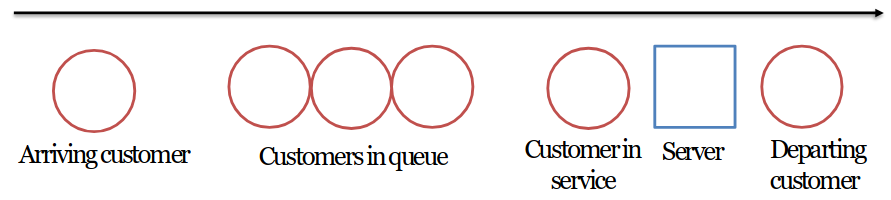
\includegraphics[width=0.8\textwidth]{images/L5.png}
    \label{fig:student_markov_chain}
\end{figure}


\subsection{Expected Average Delay in Queue}

Una delle principali misure di performance di un single-server queueing system è l’\textbf{expected average delay in queue}. Questa quantità rappresenta il tempo medio che un cliente trascorre in attesa nella coda prima di iniziare il servizio ed è quindi una misura di performance dal punto di vista del cliente.

Il valore del ritardo sperimentato dai clienti dipende direttamente dalle realizzazioni delle variabili casuali che descrivono il sistema, in particolare:
\begin{compactitemize}
    \item i tempi di interarrivo;
    \item i tempi di servizio.
\end{compactitemize}

Poiché tali grandezze sono aleatorie, anche il ritardo sperimentato da ciascun cliente è una variabile casuale. Di conseguenza, il delay medio osservato nel corso di una simulazione è esso stesso una variabile casuale, e l’obiettivo dello studio è la stima del suo \textbf{valore atteso}, indicato con $d(n)$.

Un primo estimatore naturale di questa misura è dato dalla media dei ritardi individuali osservati sui primi $n$ clienti serviti. Indicando con $D_1, D_2, \dots, D_n$ i ritardi in coda dei primi $n$ clienti, l’estimatore è definito come:
\[
\hat{d}(n) = \frac{1}{n} \sum_{i=1}^{n} D_i
\]

È importante chiarire che il termine \emph{delay} include anche il caso in cui il cliente non attenda affatto. Se un cliente arriva quando il server è idle, entra immediatamente in servizio e il suo ritardo è pari a zero. Pertanto, osservazioni con $D_i = 0$ fanno parte a pieno titolo del campione e devono essere correttamente considerate nella stima del delay medio.

Questo aspetto è rilevante dal punto di vista modellistico: stimare il delay medio senza tenere conto delle osservazioni nulle porterebbe a una valutazione distorta della performance del sistema, sovrastimando il livello di congestione percepito dai clienti.

Sebbene la forma di $\hat{d}(n)$ coincida con quella di una media aritmetica, tale estimatore non corrisponde alla ``media usuale'' della statistica classica. I ritardi individuali non sono osservazioni indipendenti e identicamente distribuite, poiché ciascun $D_i$ dipende dallo stato del sistema al momento dell’arrivo del cliente, il quale è influenzato dagli eventi precedenti.

Per questa ragione, nella pratica della simulazione a eventi discreti risulta particolarmente importante adottare estimatori che tengano esplicitamente conto dell’intera evoluzione temporale del sistema, includendo sia periodi di congestione sia periodi in cui il server è idle e i ritardi sono nulli. Solo in questo modo è possibile ottenere stime affidabili e rappresentative della reale esperienza dei clienti.

\subsection{Expected Average Queue Size}

Un’altra misura di performance fondamentale per il single-server queueing system è l’\textbf{expected average queue size}. Questa quantità rappresenta il numero medio di clienti presenti in coda ed è una misura di performance che riflette principalmente il \emph{punto di vista del manager o del decisore}, in quanto è direttamente collegata a problemi di congestione, utilizzo delle risorse e dimensionamento del sistema.

Analogamente ad altre misure di performance, il numero di clienti in coda dipende dalle realizzazioni dei tempi di interarrivo e dei tempi di servizio. Di conseguenza, anche la dimensione media della coda è una variabile casuale e l’obiettivo della simulazione è stimare il suo \textbf{valore atteso}, indicato con $q(n)$.

A differenza del delay medio, l’average queue size viene definito come una \textbf{media nel tempo}. Ciò significa che non si effettua una media sui clienti, ma si osserva come evolve nel tempo la lunghezza della coda e si calcola una media pesata rispetto alla durata dei diversi stati del sistema.

Sia $Q(t)$ il numero di clienti in coda all’istante di tempo $t$. Durante l’evoluzione della simulazione, $Q(t)$ è sempre una variabile intera non negativa. Sia inoltre $T(n)$ il tempo totale necessario per osservare i primi $n$ ritardi in coda, ovvero l’orizzonte temporale della simulazione considerata.

Per ogni istante $t$ compreso tra $0$ e $T(n)$, il processo $Q(t)$ assume valori appartenenti all’insieme $\{0,1,2,\dots\}$. Indichiamo con $p_i$ la proporzione attesa del tempo in cui la coda ha lunghezza pari a $i$, cioè la frazione di tempo in cui vale la condizione $Q(t) = i$.

L’expected average number of customers in queue può allora essere espresso come:
\[
q(n) = \sum_{i=0}^{\infty} i \cdot p_i
\]

Questa espressione mette in evidenza che $q(n)$ è una \textbf{media pesata} dei possibili valori della lunghezza della coda, in cui ogni valore $i$ è pesato dalla proporzione di tempo in cui il sistema si trova in quello stato.

Per stimare $q(n)$ tramite simulazione è quindi necessario stimare le quantità $p_i$. A tal fine, si definisce $T_i$ come il tempo totale, durante la simulazione, in cui la coda ha lunghezza pari a $i$. Un estimatore naturale di $p_i$ è dato da:
\[
\hat{p}_i = \frac{T_i}{T(n)}
\]

Sostituendo questa stima nell’espressione precedente, si ottiene l’estimatore della dimensione media della coda:
\[
\hat{q}(n) = \sum_{i=0}^{\infty} i \cdot \frac{T_i}{T(n)} = \frac{1}{T(n)} \sum_{i=0}^{\infty} i \cdot T_i
\]

Questo estimatore rappresenta il \textbf{time-average number of customers in queue}. La sua principale caratteristica è quella di tenere esplicitamente conto dell’evoluzione temporale del sistema, pesando maggiormente quegli stati della coda in cui il sistema trascorre più tempo.

Per questo motivo, la queue size media calcolata come media nel tempo fornisce una descrizione più fedele del livello di congestione del sistema rispetto a una media calcolata sui clienti, risultando particolarmente adatta per supportare decisioni di gestione e dimensionamento delle risorse.
\begin{figure}[H]
    \centering
    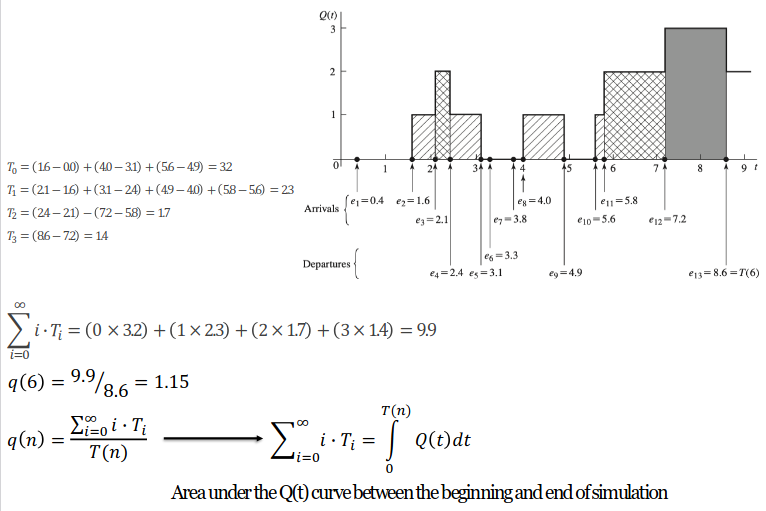
\includegraphics[width=0.9\textwidth]{images/QQ1.png}
    \label{fig:student_markov_chain}
\end{figure}

\subsection{Expected Utilization of the Server}

Un’ulteriore misura di performance fondamentale nel single-server queueing system è l’\textbf{expected utilization of the server}. Questa grandezza rappresenta la proporzione attesa di tempo durante la simulazione in cui il server risulta occupato, ovvero impegnato nell’erogazione del servizio a un cliente.

Dal punto di vista formale, l’utilization è una misura definita su \textbf{tempo continuo} ed è quindi anch’essa una variabile casuale, in quanto dipende dall’evoluzione stocastica del sistema. L’obiettivo della simulazione è stimare il valore atteso dell’utilizzazione del server, indicato con $u(n)$.

Per definire un estimatore, si introduce la funzione indicatrice $B(t)$, definita come:
\[
B(t) =
\begin{cases}
1 & \text{se il server è busy al tempo } t, \\
0 & \text{se il server è idle al tempo } t.
\end{cases}
\]

Sia inoltre $T(n)$ il tempo totale di osservazione della simulazione. Un estimatore naturale dell’utilization attesa del server è dato dalla media nel tempo di $B(t)$ sull’intervallo $[0, T(n)]$:
\[
\hat{u}(n) = \frac{1}{T(n)} \int_{0}^{T(n)} B(t)\, dt
\]

Questo estimatore rappresenta la proporzione di tempo in cui il server è stato effettivamente occupato durante la simulazione ed è noto come \textbf{continuous time-average utilization}.

L’utilization del server è una misura estremamente informativa per l’analisi delle prestazioni del sistema. Valori di utilizzo prossimi al $100\%$ indicano che il server opera quasi sempre in condizioni di saturazione. Tali situazioni sono tipicamente associate a un’elevata congestione del sistema, caratterizzata da code lunghe e ritardi medi elevati. In questo caso, il server rappresenta un potenziale \textbf{bottleneck} del sistema.

D’altra parte, livelli di utilization significativamente inferiori, ad esempio al di sotto del $90\%$, possono essere indicativi di un’eccessiva capacità installata. Questo aspetto è particolarmente rilevante quando il server rappresenta una risorsa costosa, come nel caso di robot o macchinari avanzati nei sistemi manifatturieri, dove bassi livelli di utilizzo possono tradursi in inefficienze economiche.

In conclusione, l’expected utilization of the server costituisce una misura chiave per bilanciare efficienza operativa e livello di servizio. Analizzata congiuntamente a indicatori di congestione come la queue size media e il delay medio, permette di supportare decisioni informate sul dimensionamento e la gestione delle risorse.
\begin{figure}[H]
    \centering
    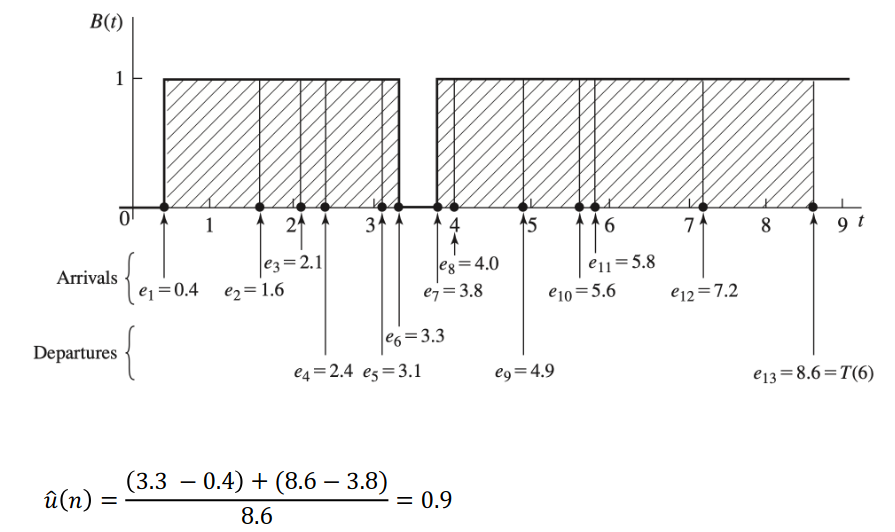
\includegraphics[width=0.8\textwidth]{images/QQ2.png}
    \label{fig:student_markov_chain}
\end{figure}

\section{Inventory System}
\subsection{Problem Statement: Inventory System}

Si considera un \textbf{sistema di gestione delle scorte} con l’obiettivo di confrontare
politiche di riordino alternative. Una società vende un singolo prodotto e deve
decidere quante unità mantenere in inventario in ciascuno dei successivi $n$ mesi,
tenendo conto dell’incertezza della domanda e dei costi associati agli ordini.

La domanda dei clienti è modellata come un processo stocastico. In particolare, i
\textbf{tempi di interarrivo della domanda} sono variabili casuali indipendenti e
identicamente distribuite (IID), con distribuzione esponenziale e valore medio pari a
$0.1$ mesi. La \textbf{dimensione della domanda} è indipendente dai tempi di arrivo ed è
descritta dalla seguente distribuzione discreta:
\[
D =
\begin{cases}
1 & \text{con probabilità } \frac{1}{6}, \\
2 & \text{con probabilità } \frac{1}{3}, \\
3 & \text{con probabilità } \frac{1}{3}, \\
4 & \text{con probabilità } \frac{1}{6}.
\end{cases}
\]

All’inizio di ciascun mese, l’azienda effettua una revisione del livello di inventario e
decide se effettuare un ordine al fornitore. Se viene effettuato un ordine di ampiezza
$Z$, il costo associato è dato da:
\[
C = K + i \cdot Z,
\]
dove $K$ rappresenta il \textbf{costo fisso di setup} dell’ordine, mentre $i$ è il
\textbf{costo incrementale unitario}. Il \textbf{lead time} (o delivery lag), ossia il
tempo che intercorre tra l’ordine e la consegna, è una variabile casuale con
distribuzione uniforme.

La politica di riordino adottata è una \textbf{politica stazionaria $(s,S)$}. Indicando
con $I$ il livello di inventario all’inizio del mese, la quantità ordinata $Z$ è definita
come:
\[
Z =
\begin{cases}
S - I & \text{se } I < s, \\
0     & \text{se } I \ge s.
\end{cases}
\]
I parametri $s$ e $S$ caratterizzano completamente la politica, mentre $Z$ rappresenta
la quantità ordinata al fornitore.

La dinamica del sistema di inventario è la seguente:
\begin{compactitemize}
    \item quando si verifica una domanda, essa viene soddisfatta immediatamente se
    il livello di inventario è sufficiente, ovvero se $I(t) \ge D_t$;
    \item se la domanda eccede il livello di inventario disponibile, l’eccesso viene
    \textbf{backlogged} e soddisfatto tramite consegne future;
    \item quando avviene una consegna, essa viene utilizzata prioritariamente per
    soddisfare eventuali arretrati di domanda; l’eventuale rimanenza viene aggiunta
    all’inventario.
\end{compactitemize}

Di conseguenza, il livello di inventario $I(t)$ può assumere sia valori positivi sia
valori negativi, a seconda della presenza di scorte o di domanda arretrata. Questo
modello consente di analizzare in modo realistico il compromesso tra costi di
ordinazione, livelli di scorta e qualità del servizio, e si presta naturalmente a uno
studio tramite simulazione per confrontare diverse politiche $(s,S)$.

\begin{figure}[H]
    \centering
    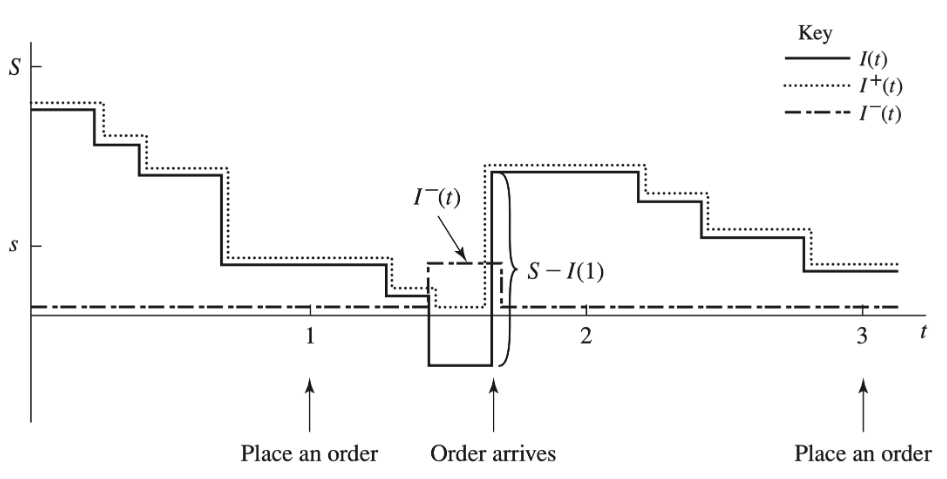
\includegraphics[width=0.8\textwidth]{images/OD10.png}
    \label{fig:student_markov_chain}
\end{figure}

\subsection{Costs}

Nel sistema di inventario considerato, le prestazioni di una politica di riordino sono
valutate sulla base dei \textbf{costi totali}, che includono costi di ordinazione,
di mantenimento delle scorte e di carenza (shortage). Tali costi sono definiti come
medie nel tempo sull’orizzonte di simulazione.

\paragraph{Ordering costs}
Quando l’azienda effettua un ordine di ampiezza $Z$, il costo di ordinazione è dato da:
\[
C = K + i \cdot Z,
\]
dove $K$ è il \textbf{costo fisso di setup} associato all’emissione dell’ordine, mentre
$i$ rappresenta il \textbf{costo incrementale unitario} per ciascun articolo ordinato.

\paragraph{Holding costs}
I costi di mantenimento delle scorte sono proporzionali al livello di inventario
positivo. Indicando con $I(t)$ il livello di inventario al tempo $t$, si definisce:
\[
I^{+}(t) = \max\{I(t), 0\}.
\]
Il costo di holding istantaneo è quindi:
\[
H(t) = h \cdot I^{+}(t),
\]
dove $h$ rappresenta il costo unitario di mantenimento. Tali costi riflettono spese
come affitto del magazzino, assicurazione, tasse, manutenzione e costi opportunità del
capitale immobilizzato.

La misura di performance associata al livello medio di scorte è definita come
\textbf{media nel tempo}:
\[
I^{+} = \frac{1}{n} \int_{0}^{n} I^{+}(t)\, dt.
\]

\paragraph{Shortage costs}
Analogamente, i costi di carenza sono legati al livello di inventario negativo, che
rappresenta la domanda arretrata (backlog). Si definisce:
\[
I^{-}(t) = \max\{-I(t), 0\}.
\]
Il costo di shortage istantaneo è:
\[
S(t) = \pi \cdot I^{-}(t),
\]
dove $\pi$ è il costo unitario di carenza, che tipicamente riflette costi di gestione,
perdita di goodwill dei clienti e potenziali mancate vendite future.

Il livello medio di backlog è anch’esso definito come media nel tempo:
\[
I^{-} = \frac{1}{n} \int_{0}^{n} I^{-}(t)\, dt.
\]

In conclusione, tutti i costi rilevanti nel sistema di inventario sono espressi come
\textbf{time-averages}, rendendo il problema particolarmente adatto a un’analisi tramite
simulazione di tipo nonterminating, finalizzata al confronto di politiche di riordino
alternative sulla base del costo medio di lungo periodo.

\subsection{Parameters}

Nel seguente studio di simulazione, il sistema di inventario è caratterizzato da un
insieme di parametri numerici fissati, che definiscono il comportamento della domanda,
dei costi e delle condizioni iniziali.

I \textbf{tempi di interarrivo della domanda} sono modellati come variabili casuali
esponenziali con valore medio pari a:
\[
E[A] = 0.1 \text{ mesi},
\]
corrispondente a un tasso medio di domanda $\mu = 0.1$.

La \textbf{dimensione della domanda} è indipendente dai tempi di arrivo ed è descritta
dalla seguente distribuzione discreta:
\[
D =
\begin{cases}
1 & \text{con probabilità } \frac{1}{6}, \\
2 & \text{con probabilità } \frac{1}{3}, \\
3 & \text{con probabilità } \frac{1}{3}, \\
4 & \text{con probabilità } \frac{1}{6}.
\end{cases}
\]

I parametri di costo associati al sistema di inventario sono:
\begin{compactitemize}
    \item costo fisso di setup dell’ordine: $K = 32$;
    \item costo incrementale unitario: $i = 3$;
    \item costo unitario di holding: $h = 1$;
    \item costo unitario di shortage: $\pi = 5$.
\end{compactitemize}

Il \textbf{lead time} del fornitore, ossia il tempo di consegna degli ordini, è una
variabile casuale uniforme con supporto:
\[
L \sim U(0.5, 1) \text{ mesi}.
\]

Il livello di inventario iniziale è fissato pari a:
\[
I(0) = 60.
\]

L’orizzonte temporale della simulazione è di:
\[
n = 120 \text{ mesi},
\]
che rappresenta un periodo sufficientemente lungo da consentire l’analisi delle
prestazioni di lungo periodo del sistema.

Questi parametri definiscono completamente l’istanza del problema di inventario
considerata e costituiscono la base per il confronto, tramite simulazione, di diverse
politiche di riordino $(s,S)$ in termini di costo medio e qualità del servizio.

\subsection{Objective}

L’obiettivo dello studio di simulazione è il confronto di un insieme di
\textbf{nove diverse politiche di inventario} di tipo stazionario $(s,S)$, al fine di
valutarne le prestazioni in termini di costo complessivo.

Le politiche considerate sono definite dalle seguenti coppie di parametri:
\[
\begin{array}{c|ccccccccc}
s & 20 & 20 & 20 & 20 & 40 & 40 & 40 & 60 & 60 \\
S & 40 & 60 & 80 & 100 & 60 & 80 & 100 & 80 & 100
\end{array}
\]

Ciascuna coppia $(s,S)$ rappresenta una diversa strategia di riordino, che bilancia in
modo differente la frequenza degli ordini, il livello medio di scorte e il rischio di
carenze.

La \textbf{misura di performance} utilizzata per il confronto tra le politiche è il
\textbf{costo totale medio mensile}, definito come:
\[
C_{\text{Tot}} = C + H + S,
\]
dove:
\begin{compactitemize}
    \item $C$ rappresenta il costo medio di ordinazione;
    \item $H$ rappresenta il costo medio di mantenimento delle scorte;
    \item $S$ rappresenta il costo medio di shortage.
\end{compactitemize}

Tutti i termini sono espressi come \textbf{medie nel tempo} sull’orizzonte di simulazione.
Il confronto tra le diverse politiche $(s,S)$ si basa quindi sul valore stimato di
$C_{\text{Tot}}$, consentendo di identificare la strategia che minimizza il costo medio
complessivo e offre il miglior compromesso tra efficienza operativa e livello di
servizio.
